\documentclass[10pt]{beamer}
\usetheme{Warsaw}

% |===| Package imports.

\usepackage{
  etex, graphicx, amssymb, amsmath, amstext, amsfonts, mathtools,
  multicol, pgfplots, array, listings, colortbl, ulem, ifthen, xcolor,
  xifthen, wrapfig
}
\usepackage[scaled=1]{beramono}
\usepackage[T1]{fontenc}
\usepackage[utf8]{inputenc}
\usepackage{tikz}

\usetikzlibrary{shapes,arrows}

\renewcommand{\baselinestretch}{1.2}

% Trying to waste less space

% \addtolength{\topmargin}{1pt}
% \addtolength{\headsep}{5pt}
% \addtolength{\oddsidemargin}{-4pt}
% \addtolength{\marginparwidth}{20pt}
% \addtolength{\marginparsep}{-3pt}
% \addtolength{\textwidth}{-5pt}


% |===| Beamer things.

% |=====| Cyan on black theme.

% |===| Basic colors.
\definecolor{background}{RGB}{0,0,0}
\definecolor{balance}{RGB}{255,255,255}
\definecolor{foreground}{RGB}{102,178,255}

% |===| Other colors.
\definecolor{cstm_red}{RGB}{255,130,130}
\definecolor{cstm_green}{RGB}{130,255,170}
\colorlet{cstm_blue}{foreground}
\definecolor{cstm_orange}{RGB}{255,180,110}
\definecolor{cstm_yellow}{RGB}{255,255,0}

% |===| Special colors.
\colorlet{daiji}{cstm_red}
\colorlet{emph}{balance}
\colorlet{code}{cstm_orange}
\colorlet{url}{balance!80!background}
\colorlet{tikz_neutral}{balance!80!background}

\setbeamercolor{normal text}{
  fg = foreground, bg = background
}
\setbeamercolor{structure}{
  fg = foreground, bg = background
}

\setbeamercolor{alerted text}{
  fg = red!85!background
}

\setbeamercolor{item projected}{
  use = item, fg = background, bg = item.fg!35!balance
}

\setbeamercolor*{palette primary}{
  use = structure, fg = structure.fg
}
\setbeamercolor*{palette secondary}{
  use = structure, fg = structure.fg!95!background
}
\setbeamercolor*{palette tertiary}{
  use = structure, fg = structure.fg!90!background
}
\setbeamercolor*{palette quaternary}{
  use = structure, fg = structure.fg!95!background, bg = background
}

\setbeamercolor*{framesubtitle}{
  fg = background!40
}

\setbeamercolor*{block title}{
  parent = structure, fg = background, bg = cstm_blue!70!balance
}
\setbeamerfont*{block title}{
  series = \bfseries
}
\setbeamercolor*{block body}{
  fg = foreground, bg = background!83!balance
}
\setbeamercolor*{block title alerted}{
  parent = alerted text, bg = background!15!balance
}
\setbeamercolor*{block title example}{
  parent = example text,bg = background!15!balance
}

\setbeamertemplate{navigation symbols}{}
\setbeamertemplate{headline}{}
\setbeamertemplate{frametitle}{
  \large\insertframetitle\hfill\small\insertsection
}
\setbeamertemplate{footline}{}
% \setbeamertemplate{footline}[frame number]{}
% \setbeamerfont{footline}{family = \rmfamily, series = \mdseries, size = \small}
% \setbeamercolor{footline}{ fg = balance }

\setbeamertemplate{itemize item}{\textbullet}


% |===| TOC things.

\AtBeginSection{
  \begin{frame}
  \frametitle{Contents}
  \tiny{\tableofcontents[hideallsubsections, currentsection]}
  \end{frame}
}

\setbeamertemplate{sections/subsections in toc}[circle]
\setbeamerfont{section in toc}{
  size = \large
}
\setbeamerfont{section number projected}{
  series = \bfseries, size = \large
}
\setbeamercolor{section number projected}{
  bg = foreground, fg = background
}

% |===| Tikz things.

% |===| Node styles.

\tikzstyle{empty} = [
  draw=none, fill=none
]

\tikzstyle{rect} = [
  draw=tikz_neutral, ultra thick, font = \bf
]
\tikzstyle{circ} = [
  rect, circle
]
\tikzstyle{elli} = [
  rect, ellipse
]

% |===| Node style modifiers.

\tikzstyle{round} = [
  rounded corners
]

\tikzstyle{drw_red}    = [ draw =    cstm_red ]
\tikzstyle{drw_green}  = [ draw =  cstm_green ]
\tikzstyle{drw_blue}   = [ draw =   cstm_blue ]
\tikzstyle{drw_orange} = [ draw = cstm_orange ]
\tikzstyle{drw_yellow} = [ draw = cstm_yellow ]

\tikzstyle{fil_red}    = [ fill =    cstm_red ]
\tikzstyle{fil_green}  = [ fill =  cstm_green ]
\tikzstyle{fil_blue}   = [ fill =   cstm_blue ]
\tikzstyle{fil_orange} = [ fill = cstm_orange ]
\tikzstyle{fil_yellow} = [ fill = cstm_yellow ]

\tikzstyle{txt_red}    = [ text =    cstm_red ]
\tikzstyle{txt_green}  = [ text =  cstm_green ]
\tikzstyle{txt_blue}   = [ text =   cstm_blue ]
\tikzstyle{txt_orange} = [ text = cstm_orange ]
\tikzstyle{txt_yellow} = [ text = cstm_yellow ]

% |===| Draw styles.

\tikzstyle{line} = [
  rect
]
\tikzstyle{arrow} = [
  rect, ->, >=latex
]

% |===| Macros.

% |===| Formatting.

\newcommand{\daiji}[1]{\textcolor{daiji}{#1}}
\newcommand{\code}[1]{{\small\texttt{\textcolor{code}{#1}}}}
\renewcommand{\emph}[1]{\textit{\textcolor{emph}{#1}}}
\newcommand{\bigsep}{\itemsep1.2em}
\newcommand{\ita}[1]{\textit{#1}}
\newcommand{\prompt}{\code{>}\xspace}
\newcommand{\impl}{\Rightarrow}
\newcommand{\daimpl}{\daiji{$\impl$}\xspace}
\newcommand{\daiheart}{\daiji{$\heartsuit$}\xspace}



% |===| Listings.

\lstdefinelanguage{rust_lst}{
  alsoletter={'},
  % backgroundcolor=\color{white},
  basicstyle = { \scriptsize\ttfamily },
%
% Lifetimes.
%
  keywords=[1]{},
  keywordstyle=[1]\color{cstm_green},
  keywordsprefix=',
%
  morekeywords=[2]{ % Orange
    struct, enum, trait, impl, use, for, while, loop, in, fn, let, pub
  },
  keywordstyle=[2]\color{cstm_orange},
%
  morekeywords=[3]{
    if, then, else, match, =>, ->
  },
  keywordstyle=[3]{\bf\ttfamily\color{foreground!70!yellow}},
%
  morekeywords=[4]{ % Types.
    Self, usize, isize, fsize,
    u8, u16, u32, u64,
    i8, i16, i32, i64,
    f8, f16, f32, f64,
    str, String, Vec, Option, Result,
    \{, \}
  },
  keywordstyle=[4]{\bf\color{balance}},
%
  morekeywords=[5]{
    mut, break, continue, return, !
  },
  keywordstyle=[5]\color{cstm_red},
%
  morekeywords=[6]{
    self
  },
  keywordstyle=[6]\color{balance!90!background},
%
  stringstyle=\color{cstm_yellow},
%
% Macros
%
  literate=*%
    {!}{{\textcolor{cstm_red}{!}}}1
    {\&}{{\textcolor{cstm_green}{\&}}}1
    {->}{{$\to$}}2,
%
% Comments
%
  morecomment=[l]{//},
  morecomment=[n]{/*}{*/},
%
  morecomment=[n][\color{balance!40!background}]{/**}{*/},
  morecomment=[n][\color{balance!40!background}]{/*!}{*/},
  morecomment=[l][\color{balance!40!background}]{///},
  morecomment=[l][\color{balance!40!background}]{//!},
%
  morestring=[b]",
  morestring=[b]""",
  % breakatwhitespace=false,
  % breaklines=true,
  % captionpos=b,
  commentstyle=\color{balance!30!background}\it\bfseries,
  % deletekeywords={...},
  % escapeinside={\%*}{*)},
  % extendedchars=true,
  frame=l,
  % keepspaces=true,
  % keywordstyle=\color{blue},
  % otherkeywords={*,...},
  % numbers=left,
  % numbersep=5pt,
  % numberstyle=\tiny\color{mygray},
  % rulecolor=\color{black},
  sensitive=true,
  % showspaces=false,
  showstringspaces=false,
  % showtabs=false,
  % stepnumber=2,
  % stringstyle=\color{mymauve},
  % tabsize=2
}
\lstnewenvironment{rust}{
  \lstset{ language = rust_lst }
}{
}

% |===| Nice links.

\hypersetup{
  colorlinks=true,
  linkcolor=url,
  urlcolor=url,
  pdftitle={Programming Language Concepts: Abstract Machines}
}


% |===| Title page info.

\title{
  Programming Language Concepts\\[3em]
  Abstract Machines\\[2em]
}

\author[]{
  Adrien Champion\\
  \href{mailto:adrien.champion@email.com}{adrien.champion@email.com}
}


\date{}

\begin{document}
\addtolength{\leftmargin}{-20pt}
\addtolength{\rightmargin}{-20pt}



\begin{frame}{}
  \titlepage
\end{frame}



\section{Languages, programs and machines}


\begin{frame}[fragile]{Notions}
  \begin{define}{programming language}{}
    a formalism with some ``instructions''
  \end{define}

  \begin{define}{program}{in language $\lang$}%
    a finite sequence of instructions in $\lang$
  \end{define}
  \pause

  \begin{define}{abstract machine}{for $\lang$}
    any set of data structures and algorithms which can perform the
    \daiji{storage and execution} of programs in $\lang$
  \end{define}
\end{frame}



\begin{frame}{Abstract machines}
  Abstract machines come in many flavors, but they share some traits.
  \bigskip

  They can
  \medskip
  \begin{itemize}
  \item process \daiji{primitive data}
  \item control the sequence of \daiji{execution of operations}
  \item control \daiji{data transfers}
  \item \daiji{manage memory}
  \end{itemize}
  \bigskip

  \pause

  More importantly they can \daiji{run}.
\end{frame}




\begin{frame}{Intuition}
  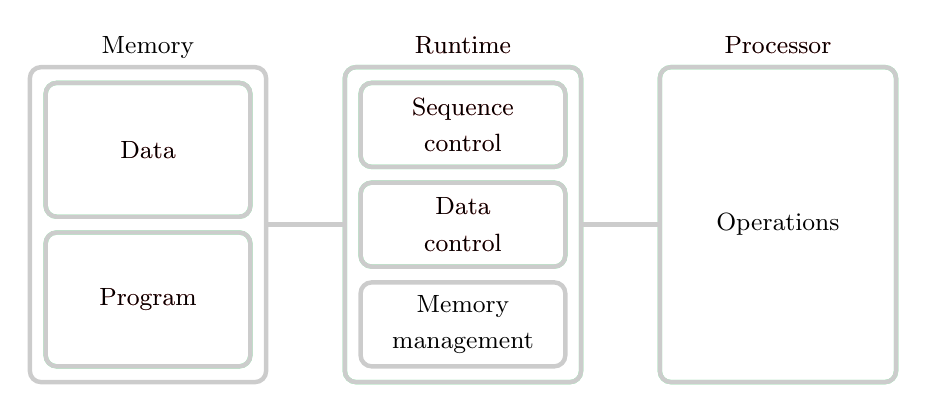
\begin{tikzpicture}

\def\hght{4}
\def\wdth{3}
\def\sep{1}
\def\inSep{.2}

\small


% |===| Memory.

\draw[rect, round]
  (0,0) -- (\wdth,0) -- (\wdth,\hght) -- (0,\hght) -- cycle ;
\node[
  empty, minimum height = 1pt, anchor = south, align = center
] () at (.5*\wdth,\hght) {Memory} ;

\def\memInWdth#1{#1*\wdth-#1*2*\inSep}
\def\memInHght#1{#1*0.5*\hght-#1*1.5*\inSep}

\alt<5,10>{
  \draw[rect, round, drw_green]
    (\inSep,\inSep) --
    (\inSep+\memInWdth{1},\inSep) --
    (\inSep+\memInWdth{1},\inSep+\memInHght{1}) --
    (\inSep,\inSep+\memInHght{1}) --
    cycle ;
  \node[empty, align = center] () at (
    \inSep+\memInWdth{.5},\inSep+\memInHght{.5}
  ) {\daiji{Program}} ;
}{
  \draw[rect, round]
    (\inSep,\inSep) --
    (\inSep+\memInWdth{1},\inSep) --
    (\inSep+\memInWdth{1},\inSep+\memInHght{1}) --
    (\inSep,\inSep+\memInHght{1}) --
    cycle ;
  \node[empty, align = center] () at (
    \inSep+\memInWdth{.5},\inSep+\memInHght{.5}
  ) {Program} ;
}

\alt<7,9>{
  \draw[rect, round, drw_green]
    (\inSep,2*\inSep+\memInHght{1}) --
    (\inSep+\memInWdth{1},2*\inSep+\memInHght{1}) --
    (\inSep+\memInWdth{1},2*\inSep+\memInHght{1}+\memInHght{1}) --
    (\inSep,2*\inSep+\memInHght{1}+\memInHght{1}) --
    cycle ;
  \node[empty, align = center] () at (
    \inSep+\memInWdth{.5},2*\inSep+\memInHght{1.5}
  ) {\daiji{Data}} ;
}{
  \draw[rect, round]
    (\inSep,2*\inSep+\memInHght{1}) --
    (\inSep+\memInWdth{1},2*\inSep+\memInHght{1}) --
    (\inSep+\memInWdth{1},2*\inSep+\memInHght{1}+\memInHght{1}) --
    (\inSep,2*\inSep+\memInHght{1}+\memInHght{1}) --
    cycle ;
  \node[empty, align = center] () at (
    \inSep+\memInWdth{.5},2*\inSep+\memInHght{1.5}
  ) {Data} ;
}


% |===| Runtime.

\uncover<2->{

  \alt<6>{
    \draw[rect, round, drw_green]
      (\sep+\wdth,0) --
      (\sep+2*\wdth,0) --
      (\sep+2*\wdth,\hght) --
      (\sep+\wdth,\hght) --
      cycle ;
    \node[
      empty, minimum height = 1pt, anchor = south, align = center
    ] () at (\sep+1.5*\wdth,\hght) {\daiji{Runtime}\vphantom{y}} ;
  }{
    \draw[rect, round]
      (\sep+\wdth,0) --
      (\sep+2*\wdth,0) --
      (\sep+2*\wdth,\hght) --
      (\sep+\wdth,\hght) --
      cycle ;
    \node[
      empty, minimum height = 1pt, anchor = south, align = center
    ] () at (\sep+1.5*\wdth,\hght) {Runtime\vphantom{y}} ;
  }

  \def\runInWdth#1{#1*\wdth-#1*2*\inSep}
  \def\runInHght#1{#1*0.333333*\hght-#1*1.333333*\inSep}

  \draw[rect, round]
    (\sep+\inSep+\wdth,\inSep) --
    (\sep+\inSep+\wdth+\runInWdth{1},\inSep) --
    (\sep+\inSep+\wdth+\runInWdth{1},\inSep+\runInHght{1}) --
    (\sep+\inSep+\wdth,\inSep+\runInHght{1}) --
    cycle ;
  \node[empty, align = center, text width = 10em] () at (
    \sep+\inSep+\wdth+\runInWdth{.5},\inSep+\runInHght{.5}
  ) {Memory\\management} ;

  \alt<5,7,9->{
    \draw[rect, round, drw_green]
      (\sep+\inSep+\wdth,2*\inSep+\runInHght{1}) --
      (\sep+\inSep+\wdth+\runInWdth{1},2*\inSep+\runInHght{1}) --
      (\sep+\inSep+\wdth+\runInWdth{1},2*\inSep+\runInHght{2}) --
      (\sep+\inSep+\wdth,2*\inSep+\runInHght{2}) --
      cycle ;
    \node[empty, align = center, text width = 10em] () at (
      \sep+\inSep+\wdth+\runInWdth{.5},2*\inSep+\runInHght{1.5}
    ) {\daiji{Data}\\\daiji{control}} ;
  }{
    \draw[rect, round]
      (\sep+\inSep+\wdth,2*\inSep+\runInHght{1}) --
      (\sep+\inSep+\wdth+\runInWdth{1},2*\inSep+\runInHght{1}) --
      (\sep+\inSep+\wdth+\runInWdth{1},2*\inSep+\runInHght{2}) --
      (\sep+\inSep+\wdth,2*\inSep+\runInHght{2}) --
      cycle ;
    \node[empty, align = center, text width = 10em] () at (
      \sep+\inSep+\wdth+\runInWdth{.5},2*\inSep+\runInHght{1.5}
    ) {Data\\control} ;
  }

  \alt<5,10>{
    \draw[rect, round, drw_green]
      (\sep+\inSep+\wdth,3*\inSep+\runInHght{2}) --
      (\sep+\inSep+\wdth+\runInWdth{1},3*\inSep+\runInHght{2}) --
      (\sep+\inSep+\wdth+\runInWdth{1},3*\inSep+\runInHght{3}) --
      (\sep+\inSep+\wdth,3*\inSep+\runInHght{3}) --
      cycle ;
    \node[empty, align = center, text width = 10em] () at (
      \sep+\inSep+\wdth+\runInWdth{.5},3*\inSep+\runInHght{2.5}
    ) {\daiji{Sequence}\\\daiji{control}} ;
  }{
    \draw[rect, round]
      (\sep+\inSep+\wdth,3*\inSep+\runInHght{2}) --
      (\sep+\inSep+\wdth+\runInWdth{1},3*\inSep+\runInHght{2}) --
      (\sep+\inSep+\wdth+\runInWdth{1},3*\inSep+\runInHght{3}) --
      (\sep+\inSep+\wdth,3*\inSep+\runInHght{3}) --
      cycle ;
    \node[empty, align = center, text width = 10em] () at (
      \sep+\inSep+\wdth+\runInWdth{.5},3*\inSep+\runInHght{2.5}
    ) {Sequence\\control} ;
  }

}


% |===| Processor.

\uncover<3->{

  \alt<8>{
    \draw[rect, round, drw_green]
      (2*\sep+2*\wdth,0) --
      (2*\sep+3*\wdth,0) --
      (2*\sep+3*\wdth,\hght) --
      (2*\sep+2*\wdth,\hght) --
      cycle ;
    \node[
      empty, anchor = south, align = center
    ] () at (2*\sep+2.5*\wdth,\hght) {\daiji{Processor}\vphantom{y}} ;
  }{
    \draw[rect, round]
      (2*\sep+2*\wdth,0) --
      (2*\sep+3*\wdth,0) --
      (2*\sep+3*\wdth,\hght) --
      (2*\sep+2*\wdth,\hght) --
      cycle ;
    \node[
      empty, anchor = south, align = center
    ] () at (2*\sep+2.5*\wdth,\hght) {Processor\vphantom{y}} ;
  }

  \node[empty, align = center] () at (
    2*\sep+2.5*\wdth,.5*\hght
  ) {Operations} ;

}


% |===| Links between stuff.

\uncover<2->{
  \draw[line] (\wdth,.5*\hght) -- (\wdth+\sep,.5*\hght) ;
}
\uncover<3->{
  \draw[line] (2*\wdth+\sep,.5*\hght) -- (2*\wdth+2*\sep,.5*\hght) ;
}


\end{tikzpicture}

  \uncover<4->{
    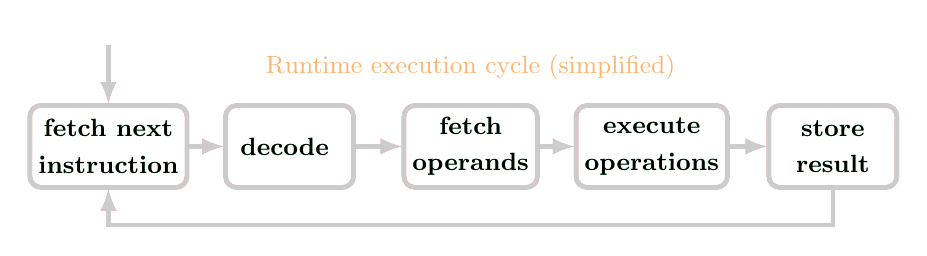
\begin{tikzpicture}

\small

\def\wdth{5}
\def\hght{3.2}
\def\sep{2.3}


\node[empty, color = cstm_orange] (title) at (2*\sep,1) {
  Runtime execution cycle (simplified)
} ;


\node[empty] (start) at (0*\sep,1.4) {} ;

\alt<5,10>{
  \node[
    rect, round, color = cstm_green, drw_red, 
    minimum width = \wdth em, minimum height = \hght em, align = center
  ] (fetch_inst) at (0*\sep,0) {
    fetch next\\instruction
  } ;
}{
  \node[
    rect, round,
    minimum width = \wdth em, minimum height = \hght em, align = center
  ] (fetch_inst) at (0*\sep,0) {
    fetch next\\instruction
  } ;
}
\alt<5>{
  \draw[arrow, drw_red] (start) -- (fetch_inst) ;
}{
  \draw[arrow] (start) -- (fetch_inst) ;
}

\alt<6>{
  \node[
    rect, round, color = cstm_green, drw_red,
    minimum width = \wdth em, minimum height = \hght em, align = center
  ] (decode) at (1*\sep,0) {
    decode
  } ;
  \draw[arrow, drw_red] (fetch_inst) -- (decode) ;
}{
  \node[
    rect, round,
    minimum width = \wdth em, minimum height = \hght em, align = center
  ] (decode) at (1*\sep,0) {
    decode
  } ;
  \draw[arrow] (fetch_inst) -- (decode) ;
}

\alt<7>{
  \node[
    rect, round, color = cstm_green, drw_red,
    minimum width = \wdth em, minimum height = \hght em, align = center
  ] (fetch_op) at (2*\sep,0) {
    fetch\\operands
  } ;
  \draw[arrow, drw_red] (decode) -- (fetch_op) ;
}{
  \node[
    rect, round,
    minimum width = \wdth em, minimum height = \hght em, align = center
  ] (fetch_op) at (2*\sep,0) {
    fetch\\operands
  } ;
  \draw[arrow] (decode) -- (fetch_op) ;
}

\alt<8>{
  \node[
    rect, round, color = cstm_green, drw_red,
    minimum width = \wdth em, minimum height = \hght em, align = center
  ] (execute) at (3*\sep,0) {
    execute\\operations
  } ;
  \draw[arrow, drw_red] (fetch_op) -- (execute) ;
}{
\node[
    rect, round,
    minimum width = \wdth em, minimum height = \hght em, align = center
  ] (execute) at (3*\sep,0) {
    execute\\operations
  } ;
  \draw[arrow] (fetch_op) -- (execute) ;
}

\alt<9>{
  \node[
    rect, round, color = cstm_green, drw_red,
    minimum width = \wdth em, minimum height = \hght em, align = center
  ] (store) at (4*\sep,0) {
    store\\result
  } ;
  \draw[arrow, drw_red] (execute) -- (store) ;
}{
  \node[
    rect, round,
    minimum width = \wdth em, minimum height = \hght em, align = center
  ] (store) at (4*\sep,0) {
    store\\result
  } ;
  \draw[arrow] (execute) -- (store) ;
}

\alt<10>{
  \draw[arrow, drw_red]
    (store.south) --
    (4*\sep,-1) --
    (0*\sep,-1) --
    (fetch_inst.south) ;
}{
  \draw[arrow]
    (store.south) --
    (4*\sep,-1) --
    (0*\sep,-1) --
    (fetch_inst.south) ;
}


\end{tikzpicture}
  }
\end{frame}



\begin{frame}{Runtime}
  As we saw, the runtime
  \smallskip
  \begin{itemize}
  \item decides which instruction to execute next,
  \item fetches the \daiji{instruction},
  \item decodes it in terms of \daiji{primitive operations},
  \item fetches the \daiji{operands},
  \item \daiji{executes} the primitive operations,
  \item stores the \daiji{result}.
  \end{itemize}

  \bigskip
  \pause

  What about \emph{memory management}?
\end{frame}




\begin{frame}{Memory management}
  It can
  \smallskip
  \begin{itemize}
  \item \emph{allocate} / \emph{free} memory,
  \item handle the \emph{heap} / \emph{stack} (if any),
  \item do garbage collection,
  \item \emph{suspend} the execution of a program.
  \end{itemize}

  \pause
  \bigskip

  Ranges from simple to very complex depending on the abstract machine.
\end{frame}




\section{Organic example: mictyris guinotae}


\begin{frame}{Soldier crabs}
  \begin{minipage}{.5\textwidth}
  Soldier crabs crossing path have a\\\daiji{deterministic} behavior
  \\\smallskip
  We can \daiji{build circuits} as lanes
  \end{minipage}~\begin{minipage}{.49\textwidth}
    \begin{center}
      \begin{tikzpicture}
        \def\sep{7}
        \node [inner sep=0pt] at (0,0) {
          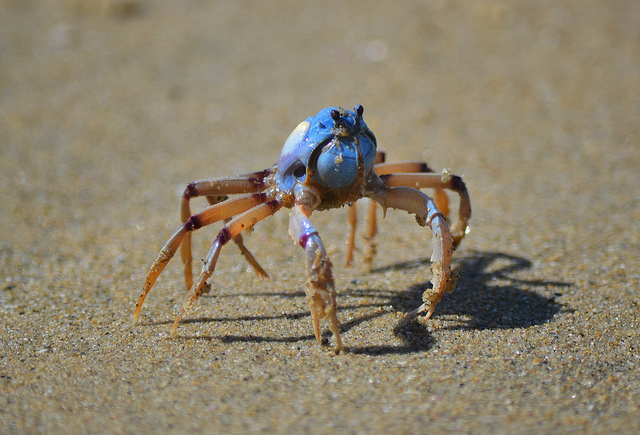
\includegraphics[width = \textwidth]{soldier_crab}
        } ;
        \draw [
          draw = bg, rounded corners=\sep, line width=\sep
        ] (current bounding box.north west) -- 
          (current bounding box.north east) --
          (current bounding box.south east) --
          (current bounding box.south west) --
          cycle ;
      \end{tikzpicture}\\
      {\tiny
        \url{http://www.gizmag.com/crab-computer-kobe/22145/}\\
        \url{http://arxiv.org/pdf/1204.1749v1.pdf}
      }
    \end{center}
  \end{minipage}
  \pause
  \begin{center}
    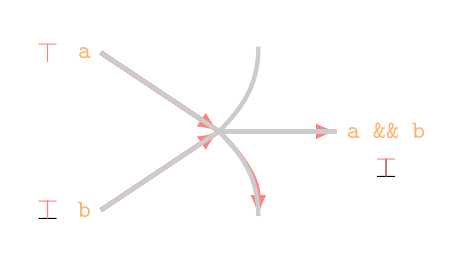
\begin{tikzpicture}

% |===| AND gate.

\node[empty, anchor = east] (a) at (0,2) {\code{a}} ;
\node[empty, anchor = east] (b) at (0,0) {\code{b}} ;
\node[empty, anchor = west] (c) at (3,1) {\code{a \&\& b}} ;

\uncover<3->{
  \node[empty, anchor = east] () at (a.west) {\daiji{\textbf{$\top$}}} ;
} ;
\uncover<3-6>{
  \node[empty, anchor = east] () at (b.west) {\textbf{$\bot$}} ;
} ;
\uncover<7->{
  \node[empty, anchor = east] () at (b.west) {\daiji{\textbf{$\top$}}} ;
} ;
\uncover<6>{
  \node[empty, anchor = north] () at (c.south) {\textbf{$\bot$}} ;
} ;
\uncover<10>{
  \node[empty, anchor = north] () at (c.south) {\daiji{\textbf{$\top$}}} ;
} ;

\alt<4-6>{
  \alt<5->{
    \draw[line, drw_red] (a.east) -- (1.5,1) ;
  }{
    \draw[arrow, drw_red] (a.east) -- (1.5,1) ;
  }
}{
  \alt<8->{
    \alt<9->{
      \draw[line, drw_red] (a.east) -- (1.5,1) ;
    }{
      \draw[arrow, drw_red] (a.east) -- (1.5,1) ;
    }
  }{
    \draw[line] (a.east) -- (1.5,1) ;
  }
}
\alt<8->{
  \alt<9->{
    \draw[line, drw_red] (b.east) -- (1.5,1) ;
  }{
    \draw[arrow, drw_red] (b.east) -- (1.5,1) ;
  }
}{
  \draw[line] (b.east) -- (1.5,1) ;
}
\alt<9->{
  \draw[arrow, drw_red] (1.5,1) -- (c.west) ;
}{
  \draw[line] (1.5,1) -- (c.west) ;
}

\node[empty] (void1) at (2,2.2) {} ;
\node[empty] (void2) at (2,-.2) {} ;

\draw[line] (1.5,1) to[out = 45, in = -90] (void1) ;
\alt<5-6>{
  \draw[arrow, drw_red] (1.5,1) to[out = -45, in = 90] (void2) ;
}{
  \draw[line] (1.5,1) to[out = -45, in = 90] (void2) ;
} ;

\end{tikzpicture}
  \end{center}
\end{frame}



\begin{frame}{Soldier crabs (runtime)}
  \daiji{Sequence control / data transfer:} humans put crabs in lanes
  \\\bigskip
  \daiji{Processing primitive data:} only \code{bool} is supported
  \begin{itemize}
  \item \code{true}: a least a crab in the lane
  \item \code{false}: no crab in the lane
  \item processor: lanes (circuit) powered by crab legs and brain
  \end{itemize}
  \bigskip
  \pause
  Although it is \daiji{silly}, can we (at least in theory)
  \begin{itemize}
  \item do \daiji{arithmetic}? How?
  \item implement sequence control / data transfer?
  \end{itemize}
\end{frame}




\section{Hardware example}



\begin{frame}{Memory}
  Memory:
  \begin{itemize}
  \item composed of \emph{RAM}, \emph{caches} (L1, L2, L3), \ldots
  \item stores \emph{words} of $32$ / $64$ bits
  \item recognizes \daiji{primitive types}
    (\textit{a.k.a.} \daiji{predefined types}):\\
    booleans, integers, floats, characters, fixed-length sequences, \ldots
  \end{itemize}
\end{frame}


\begin{frame}{Language}
  Composed of simple instructions:
  \centerline{\code{OpCode} \code{Operand1} \code{Operand2}}

  \smallskip
  For instance:
  \begin{itemize}
  \item add the \daiji{contents of registers} \code{R0} and \code{R5}, store result
    in \code{R5}:\\
    \centerline{\code{ADD} \code{R5} \code{R0}}
  \item add the contents of the \daiji{memory cells} whose \daiji{addresses}
    are stored in registers \code{R0} and \code{R5}, store result in the cell
    \code{R5} \daiji{points to}:\\
    \centerline{\code{ADD} \code{(R5)} \code{(R0)}}
  \end{itemize}
\end{frame}


\begin{frame}{Runtime}
  \daiji{Sequence control:} \emph{Program Counter (PC)} (special register)
  \begin{itemize}
  \item contains the address of the \daiji{next instruction} to execute
  \item supports operations like \emph{increment}, \emph{jump}, \ldots
  \end{itemize}
  \bigskip
  \daiji{Processing primitive data:} \emph{Arithmetic and Logic Unit (ALU)}
  \begin{itemize}
  \item arithmetic (\code{int}, \code{float}) and logical (\code{bool})
    operations
  \end{itemize}
  \bigskip
  \daiji{Data transfer:}
  \begin{itemize}
  \item special registers (MAR / MDR) bridge the memory / CPU gap
  \item handles different \emph{addressing modes}
  \item operations to load data in the CPU's registers are provided
  \end{itemize}
\end{frame}




\section{Implementation}



\begin{frame}{Trade-off}
  Implementing a machine for a language is a trade-off between
  \begin{itemize}
  \item \daiji{performance}
  \item \daiji{flexibility} -- when the language evolves
  \item \daiji{portability} -- diffusion of \emph{executables}
  \end{itemize}
  \bigskip
  Eventually, code will run on a \emph{physical} machine, the \daiji{hardware}.
  \pause
  \\\bigskip
  Hardware-level is the reference \daiji{performance-wise}:\\
  can't go faster than hardware by definition.
\end{frame}


\begin{frame}{Implementation levels}
  \daiji{Hardware}
  \begin{itemize}
  \item very fast
  \item need to build new machines when language changes
  \item can't share executable with different machines
  \end{itemize}
  \bigskip
  \daiji{Software}
  \begin{itemize}
  \item very slow (compared to hardware) (why?)
  \item easy to propagate changes in the language
  \item can share with different machines (if runtime installed)
  \end{itemize}
  \bigskip
  \daiji{Firmware}\\
  compromise between hardware and software
\end{frame}



\end{document}
